% Source-faithful schematic draft: 2004 Hunan Science Q22, PDF p.2 (printed p.175).
% Source ID: src-9f80071b553ab4b942482c92509eda24ffc4990bd51cd38172372a29634438da
% Source SHA-256: 47ba4497f88a0667fcfd694f4b8a9a37e7b1d3f098a0ad26b0529b990194e2c7
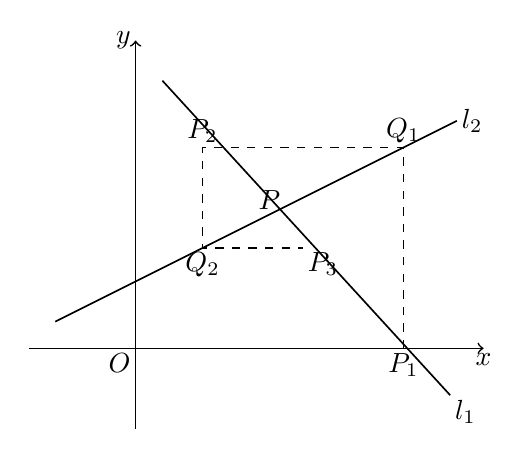
\begin{tikzpicture}[line width=0.6pt,scale=1.7,every node/.style={inner sep=1.5pt}]
  % Axes
  \draw[->] (-0.8, 0) -- (2.6, 0) node[below] {$x$};
  \draw[->] (0, -0.6) -- (0, 2.3) node[left] {$y$};
  \node[below left] at (0, 0) {$O$};

  % Coordinates based on k = -1:
  % P(1, 1), l1: y = -x + 2, l2: y = 0.5x + 0.5
  \coordinate (P) at (1, 1);
  \coordinate (P1) at (2, 0);
  \coordinate (Q1) at (2, 1.5);
  \coordinate (P2) at (0.5, 1.5);
  \coordinate (Q2) at (0.5, 0.75);
  \coordinate (P3) at (1.25, 0.75);

  % Line l1
  \draw[line width=0.6pt] (0.2, 2.0) -- (2.35, -0.35) node[below right] {$l_1$};

  % Line l2
  \draw[line width=0.6pt] (-0.6, 0.2) -- (2.4, 1.7) node[right] {$l_2$};

  % Dashed staircase lines
  \draw[dashed, line width=0.5pt] (P1) -- (Q1) -- (P2) -- (Q2) -- (P3);

  % Labels
  \node[above] at (P) {$P$};
  \node[below] at (P1) {$P_1$};
  \node[above] at (Q1) {$Q_1$};
  \node[above] at (P2) {$P_2$};
  \node[below] at (Q2) {$Q_2$};
  \node[below right] at (P3) {$P_3$};
\end{tikzpicture}
